\section{Busybox}

\begin{frame}
  \frametitle{Why Busybox?}
  \begin{itemize}
  \item A Linux system needs a basic set of programs to work
    \begin{itemize}
    \item An init program
    \item A shell
    \item Various basic utilities for file manipulation and system
      configuration
    \end{itemize}
  \item In normal GNU/Linux systems, these programs are provided by
    different projects
    \begin{itemize}
    \item \code{coreutils}, \code{bash}, \code{grep}, \code{sed},
      \code{tar}, \code{wget}, \code{modutils}, etc. are all different
      projects
    \item A lot of different components to integrate
    \item Components not designed with embedded systems constraints in
      mind: they are not very configurable and have a wide range of
      features
    \end{itemize}
  \item Busybox is an alternative solution, extremely common on
    embedded systems
  \end{itemize}
\end{frame}

\begin{frame}
  \frametitle{General purpose toolbox: BusyBox}
  \begin{columns}
    \column{0.75\textwidth}
      \url{https://www.busybox.net/}
      \begin{itemize}
      \item Rewrite of many useful UNIX command line utilities
        \begin{itemize}
        \item Created in 1995 to implement a rescue and installer
         system for Debian, fitting in a single floppy disk (1.44 MB)
        \item Integrated into a single project, which makes it easy to
          work with
        \item Designed with embedded systems in mind: highly configurable,
          no unnecessary features
        \item Called the {\em Swiss Army Knife of Embedded Linux}
        \end{itemize}
      \item License: GNU GPLv2
      \item Alternative: Toybox, BSD licensed (\url{https://en.wikipedia.org/wiki/Toybox})
      \end{itemize}
    \column{0.25\textwidth}
    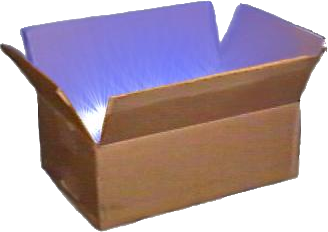
\includegraphics[width=\textwidth]{common/busybox.png}
  \end{columns}
\end{frame}

\begin{frame}
  \frametitle{BusyBox in the root filesystem}
  \begin{columns}
    \column{0.65\textwidth}
      \begin{itemize}
      \item All the utilities are compiled into a single executable,
        \code{/bin/busybox}
        \begin{itemize}
        \item Symbolic links to \code{/bin/busybox} are created for each
          application integrated into Busybox
        \end{itemize}
      \item For a fairly featureful configuration, less than 500 KB
        (statically compiled with uClibc) or less than 1 MB (statically
        compiled with glibc).
      \end{itemize}
    \column{0.35\textwidth}
      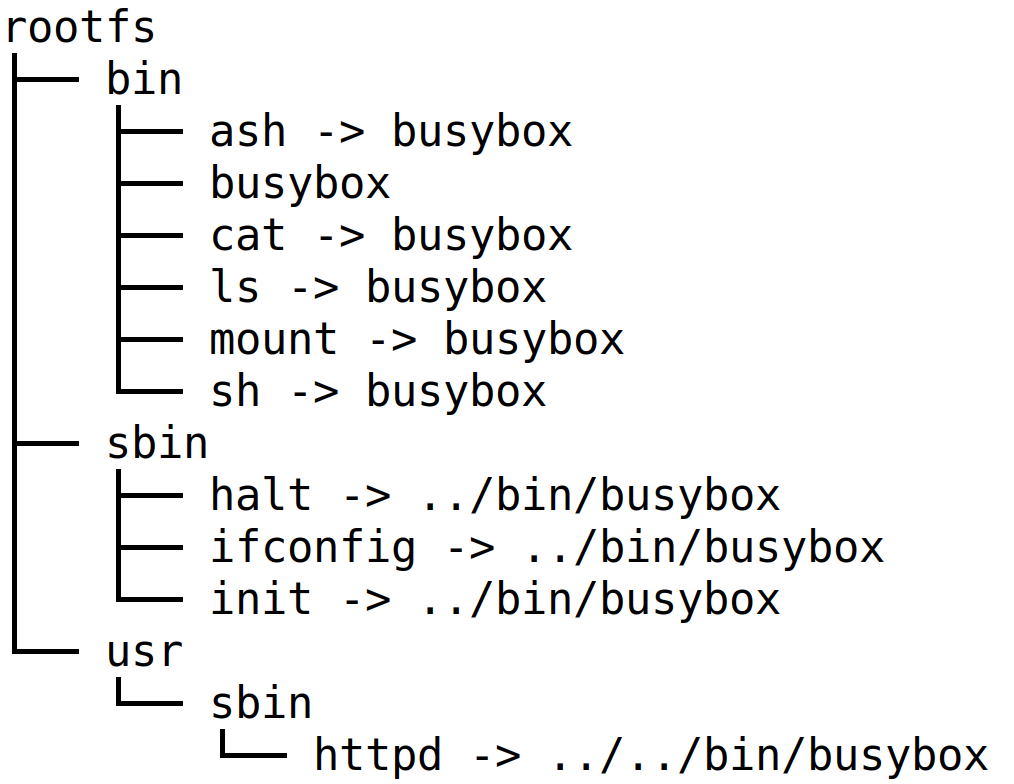
\includegraphics[width=\textwidth]{slides/sysdev-busybox/busybox-tree.png}
  \end{columns}
\end{frame}

\begin{frame}
  \frametitle{BusyBox commands!}
  \begin{spacing}{0}
    \tiny
    \code{[, [[, acpid, add-shell, addgroup, adduser, adjtimex, ar,
arch, arp, arping, awk, base64, basename, bbconfig, bc, beep,
blkdiscard, blkid, blockdev, bootchartd, brctl, bunzip2, busybox, bzcat,
bzip2, cal, cat, chat, chattr, chcon, chgrp, chmod, chown, chpasswd,
chpst, chroot, chrt, chvt, cksum, clear, cmp, comm, conspy, cp, cpio,
crond, crontab, cryptpw, cttyhack, cut, date, dc, dd, deallocvt,
delgroup, deluser, depmod, devmem, df, diff, dirname, dmesg, dnsd,
dnsdomainname, dos2unix, dpkg, dpkg-deb, du, dumpkmap, dumpleases, echo,
ed, egrep, eject, env, envdir, envuidgid, ether-wake, expand, expr,
factor, fakeidentd, fallocate, false, fatattr, fbset, fbsplash, fdflush,
fdformat, fdisk, fgconsole, fgrep, find, findfs, flash_eraseall,
flash_lock, flash_unlock, flashcp, flock, fold, free, freeramdisk, fsck,
fsck.minix, fsfreeze, fstrim, fsync, ftpd, ftpget, ftpput, fuser,
getenforce, getopt, getsebool, getty, grep, groups, gunzip, gzip, halt,
hd, hdparm, head, hexdump, hexedit, hostid, hostname, httpd, hush,
hwclock, id, ifconfig, ifdown, ifenslave, ifplugd, ifup, inetd, init,
insmod, install, ionice, iostat, ip, ipaddr, ipcalc, ipcrm, ipcs,
iplink, ipneigh, iproute, iprule, iptunnel, kbd_mode, kill, killall,
killall5, klogd, last, less, link, linux32, linux64, linuxrc, ln,
load_policy, loadfont, loadkmap, logger, login, logname, logread,
losetup, lpd, lpq, lpr, ls, lsattr, lsmod, lsof, lspci, lsscsi, lsusb,
lzcat, lzma, lzop, lzopcat, makedevs, makemime, man, matchpathcon,
md5sum, mdev, mesg, microcom, minips, mkdir, mkdosfs, mke2fs, mkfifo,
mkfs.ext2, mkfs.minix, mkfs.reiser, mkfs.vfat, mknod, mkpasswd, mkswap,
mktemp, modinfo, modprobe, more, mount, mountpoint, mpstat, mt, mv,
nameif, nanddump, nandwrite, nbd-client, nc, netcat, netstat, nice, nl,
nmeter, nohup, nologin, nproc, nsenter, nslookup, ntpd, nuke, od,
openvt, partprobe, passwd, paste, patch, pgrep, pidof, ping, ping6,
pipe_progress, pivot_root, pkill, pmap, popmaildir, poweroff, printenv,
printf, ps, pscan, pstree, pwd, pwdx, raidautorun, rdate, rdev,
readahead, readlink, readprofile, realpath, reboot, reformime,
remove-shell, renice, reset, resize, restorecon, resume, rev, rfkill,
rm, rmdir, rmmod, route, rpm, rpm2cpio, rtcwake, run-init, run-parts,
runcon, runlevel, runsv, runsvdir, rx, script, scriptreplay, sed,
selinuxenabled, sendmail, seq, sestatus, setarch, setconsole,
setenforce, setfattr, setfiles, setfont, setkeycodes, setlogcons,
setpriv, setsebool, setserial, setsid, setuidgid, sh, sha1sum,
sha256sum, sha3sum, sha512sum, showkey, shred, shuf, slattach, sleep,
smemcap, softlimit, sort, split, ssl_client, start-stop-daemon, stat,
strings, stty, su, sulogin, sum, sv, svc, svlogd, svok, swapoff, swapon,
switch_root, sync, sysctl, syslogd, tac, tail, tar, taskset, tc, tcpsvd,
tee, telnet, telnetd, test, tftp, tftpd, time, timeout, top, touch, tr,
traceroute, traceroute6, true, truncate, ts, tty, ttysize, tunctl,
tune2fs, ubiattach, ubidetach, ubimkvol, ubirename, ubirmvol, ubirsvol,
ubiupdatevol, udhcpc, udhcpd, udpsvd, uevent, umount, uname, uncompress, unexpand, uniq,
unit, unix2dos, unlink, unlzma, unlzop, unxz, unzip, uptime, users,
usleep, uudecode, uuencode, vconfig, vi, vlock, volname, w, wall, watch,
watchdog, wc, wget, which, who, whoami, whois, xargs, xxd, xz, xzcat,
yes, zcat, zcip}
  \end{spacing}
  \vfill
  Source: run \code{/bin/busybox}
\end{frame}

\begin{frame}
  \frametitle{Configuring BusyBox}
  \begin{itemize}
  \item Get the latest stable sources from \url{https://busybox.net}
  \item Configure BusyBox (creates a \code{.config} file):
    \begin{itemize}
    \item \code{make defconfig}\\
      Good to begin with BusyBox.\\
      Configures BusyBox with all options for regular users.
    \item \code{make allnoconfig}\\
      Unselects all options. Good to configure only what you need.
    \end{itemize}
  \item \code{make menuconfig} (text)\\
    Same configuration interfaces as the ones used by the Linux kernel
    (though older versions are used, causing \code{make xconfig} to
    be broken in recent distros).
  \end{itemize}
\end{frame}

\begin{frame}
  \frametitle{BusyBox make menuconfig}
  \begin{columns}
    \column{0.5\textwidth}
    You can choose:
    \begin{itemize}
    \item the commands to compile,
    \item and even the command options and features that you need!
    \end{itemize}
    \column{0.5\textwidth}
    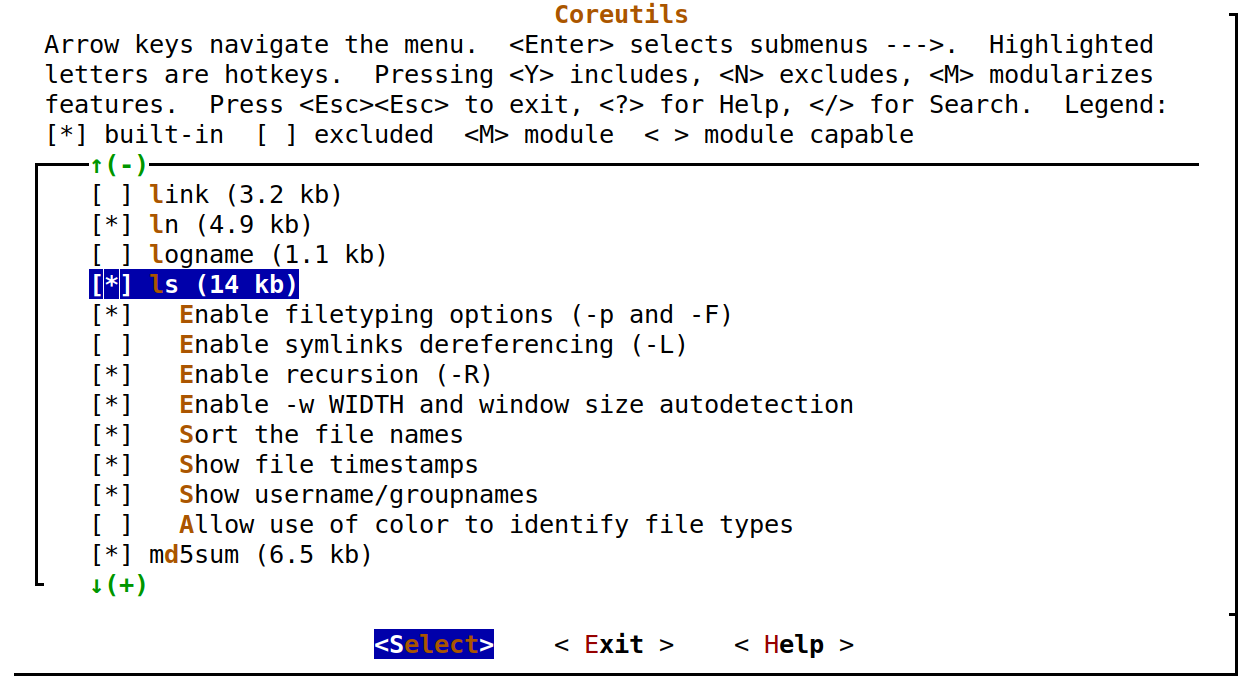
\includegraphics[width=\textwidth]{slides/sysdev-busybox/menuconfig-screenshot.png}
  \end{columns}
\end{frame}

\begin{frame}
  \frametitle{Compiling BusyBox}
  \begin{itemize}
  \item Set the cross-compiler prefix in the configuration interface: \\
    \code{Settings ->  Build Options ->  Cross Compiler
      prefix}\\
    Example: \code{arm-linux-}
  \item Set the installation directory in the configuration interface: \\
    \code{Settings ->  Installation Options ->  BusyBox
      installation prefix}
  \item Add the cross-compiler path to the PATH environment variable:\\
    \code{export PATH=$HOME/x-tools/arm-unknown-linux-uclibcgnueabi/bin:$PATH}
  \item Compile BusyBox:\\
    \code{make}
  \item Install it (this creates a UNIX directory structure symbolic
    links to the \code{busybox} executable):\\
    \code{make install}
  \end{itemize}
\end{frame}

\begin{frame}
  \frametitle{Applet highlight: Busybox init}
  \begin{itemize}
  \item Busybox provides an implementation of an \code{init} program
  \item Simpler than the init implementation found on desktop/server
    systems ({\em SysV init} or {\em systemd})
  \item A single configuration file: \code{/etc/inittab}
    \begin{itemize}
    \item Each line has the form \code{<id>::<action>:<process>}
    \end{itemize}
  \item Allows to run services at startup, and to make sure that
    certain services are always running on the system
  \item See \projfile{busybox}{examples/inittab} in Busybox for details on the
    configuration
  \end{itemize}
\end{frame}

\begin{frame}
  \frametitle{Applet highlight - BusyBox vi}
  \begin{columns}
    \column{0.6\textwidth}
      \begin{itemize}
      \item If you are using BusyBox, adding \code{vi} support only adds
        about 20K
      \item You can select which exact features to compile in.
      \item Users hardly realize that they are using a lightweight \code{vi}
        version!
      \item Tip: you can learn \code{vi} on the desktop, by running the \code{vimtutor}
        command.
      \end{itemize}
    \column{0.4\textwidth}
      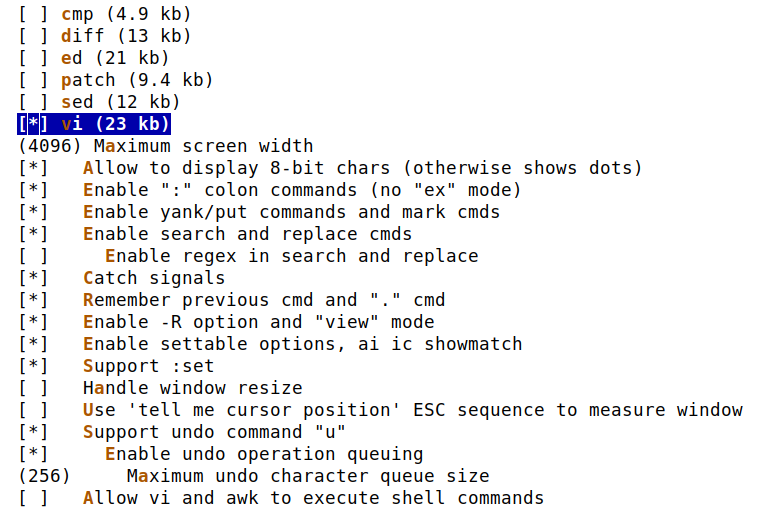
\includegraphics[width=\textwidth]{slides/sysdev-busybox/busybox-vi-configuration.png}
  \end{columns}
\end{frame}

\setuplabframe
{A tiny embedded system}
{
  \begin{itemize}
  \item Make Linux boot on a directory on your workstation, shared by NFS
  \item Create and configure a minimalistic Linux embedded system
  \item Install and use BusyBox
  \item System startup with \code{/sbin/init}
  \item Set up a simple web interface
  \item Use shared libraries
  \end{itemize}
}

\quizframe
{Filesystem and BusyBox}
{Test your understanding of the Linux root filesystem and BusyBox}
{https://frama.link/GSajeUbB}
